
\section{Overview of PlinyCompute}

We give an overview of PlinyCompute, focusing on the core components of the
system: the PC object model, 
the PC API and TCAP compiler, and execution engine, and we concretize these ideas by
describing the implementation of a simple $k$-means clustering algorithm.

\subsection{The PC Object Model}

There is growing evidence that the CPU cost associated with manipulating data, especially data (de-)serialization and memory 
(de-)allocation,  
dominate the time needed to complete typical big data processing tasks
\cite{ousterhout2015making, shi2015clash}.
To avoid these potential pitfalls while at the same time giving the user a high degree of flexibility,
PC requires programmers to store and manipulate data using the \emph{PC object model}.
The PC object model is an API for storing and manipulating persistent
data, and has been co-designed with PC's memory management system and computational engine to provide
maximum performance.  

In PC's C++ binding, individual PC \texttt{Object}s correspond to C++ objects, and so the C++ compiler specifies the memory layout.
However, where PC \texttt{Object}s are stored in RAM and on disk, and how they are allocated and deallocated, when and where they are moved, is
tightly controlled by PC itself.

The PC object model provides a fully object-oriented interface, and yet manages to avoid many of the costs associated with complex object manipulation
by following the \emph{page as a heap} principle.  
All PC \texttt{Object}s are allocated and manipulated in-place, on a system-
(or user-) allocated page.  There is
no distinction between the in-memory representation of data and the on-disk (or in-network) representation of
data. Thus there is no (de-)serialization cost to move data to/from disk and network, and memory management costs are very low. Depending upon choices made by the
programmer, ``deallocating'' a page of records
may mean simply writing over the page with a new page of records.  
In computer systems design, this is often referred to as
\emph{region-based allocation} \cite{tofte1997region,
  grossman2002region}, and is often the fastest way to manage
memory. 
TCAP query processing engine follows this strategy by pinning a page from the buffer
pool for object creation and manipulation, and unpinning the page once
it finishes manipulating on the objects allocated in that page.

To illustrate use of the PC object model from a user's perspective,
imagine that we wish to perform a computation over a number of one-dimensional feature vectors.  
Using the PC object model's C++ binding, we might represent each data point using the 
\texttt{DataPoint} class:

\begin{codesmall}
class DataPoint : public Object {
public:
	Handle <Vector <double>> data;
};
\end{codesmall}

\noindent
To create a load such data into a PC compute cluster, we might write the following code:

\begin{codesmall}
makeObjectAllocatorBlock (1024 * 1204);
Handle <Vector <Handle <DataPoint>>> myVec = 
     makeObject <Vector <Handle <DataPoint>>> ();
Handle <DataPoint> storeMe = makeObject <DataPoint> ();
storeMe->data = makeObject <Vector <double>> ();

for (int i = 0; i < 100; i++) 
     storeMe->data->push_back (1.0 * i);

myVec->push_back (storeMe);
pcContext.createSet <DataPoint> ("Mydb", "Myset");
pcContext.sendData <DataPoint> ("Mydb", "Myset", myVec);
\end{codesmall}

\noindent
Here, the programmer starts out by creating a one megabyte \emph{allocation block} where all new objects will be written,
and then allocates data directly to that allocation block via a call to \texttt{makeObject ()}.  Each call to  \texttt{makeObject ()}
returns PC's pointer-like object, called a \texttt{Handle}.  PC \texttt{Handle}s use offsets rather than an absolute memory
address, so they can be moved from process to process and remain valid.  

When the data are dispatched via \texttt{sendData ()},
the occupied
portion of the allocation block is transferred in its entirety with
no pre-processing and zero CPU cost, aside from the cycles required to perform the data transfer.  
This illustrates the principle of \emph{zero cost data movement}.

To achieve high performance, all memory management except buffer pool
page management is taken care of by the PC object model.
If the next line of code executed were:
\texttt{
myVec = nullptr;}
then all of the memory associated with the \texttt{Vector} of \texttt{DataPoint} objects would be automatically
freed, since PC \texttt{Object}s are reference counted.  This can
be expensive, however, since the PC \texttt{Object} infrastructure must traverse a potentially large graph of \texttt{Handle} objects to perform the deallocation.  
Recognizing that low-level data manipulations dominate big data
compute times \cite{ousterhout2015making, shi2015clash}, PlinyCompute gives a programmer nearly complete control
over most aspects of memory management.

If the 
programmer had instead used: 

\begin{code}
storeMe->data = makeObject <Vector <double>> (ObjectPolicy :: noRefCount);
\end{code}


\noindent then the memory associated with \texttt{storeMe->data} would
not be reference counted, and hence not reclaimed when no longer
reachable.  

This may mean lower memory utilization,
but the benefit is nearly zero-CPU-cost memory management within the block.
PC gives the developer the ability to manage the tradeoff.
This illustrates another key principle behind the design of
PlinyCompute: \emph{Since PC is targeted towards tool and library
  development, PC assumes the programmer knows what s/he is doing.  In
  the small, PC gives the programmer all of the tools s/he needs to make things fast}.

Finally, we note that the PC object model is not used exclusively or
even primarily for application programming.  The PC object model
is used \emph{internally}, with PC's computational engine as well.
For example, aggregation is implemented using PC's built-in
\texttt{Map} class.  Each thread maintains
a \texttt{Map} object that it aggregates its local data to; those are
merged into maps that are sent to various workers around the PC
cluster.  All sends and receives of these \texttt{Map} objects happen
without (de-)serialization, with zero CPU cost, aside from the CPU
cycles needed to transmit the bytes.



\subsection{PlinyCompute's Computational Engine}
\label{sec:engine}

Volcano-style, record-by-record iteration \cite{graefe1990encapsulation} has fallen out of favor over the last decade, largely replaced by
two competing paradigms for processing data
in high-performance, data-oriented computing.  The first is \emph{vectorized} processing \cite{abadi2009column, boncz2005monetdb, zukowski2005monetdb, idreos2012monetdb}, where a column of values are pushed
through a simple computation in sequence, so as to play to the strength of a modern CPU, with few cache misses and no virtual
function calls.  The second is \emph{code generation} \cite{neumann2011efficiently, nagel2014code, bress2017generating, klonatos2014building, ahmad2009dbtoaster}, where a system analyzes the computation
and then generates code---either C/C++ code, or byte code for a framework such as LLVM \cite{lattner2004llvm, lattner2002llvm}.

While PlinyCompute certainly leverages ideas from both camps, we argue that the ``vectorized vs. generated'' argument is relevant mostly for 
relational systems with a data-oriented, domain-specific language (such as SQL).  
The data manipulations directly specified by an SQL programmer are likely to be limited, 
consisting of comparison between attributes, simple arithmetic, and logical operations.
Applying classical vectorization to PC,
which requires an execution plan to be constructed consisting entirely of calls to a toolkit of
vector-based operations shipped with the system, is
unrealistic when most/all computations are over user-defined types.  Code generation---at least as described in the database literature---is also
unrealistic in such an environment.  Generating LLVM code for complex operations over user-defined types 
in a high-level language 
is akin to writing a full-fledged compiler. 


PC uses a hybrid approach, where the PC execution engine is vectorized, but where the code for the individual vectorized operations (called \emph{pipeline stages})
are fully compiled.  
In PC, a user does not specify the graph of pipeline stages directly.  Rather,
the programmer expresses her/his intent at a high-level, by building a graph of high-level operations.  These operations tend to be much higher
level than those provided by other platforms, and, like in a relational database engine, are not associated with any specific 
physical implementation.
For example, PC supplies an abstract $n$-way join called a \texttt{JoinComp}.

Operations are customized when a user supplies a set of 
\emph{lambda term
construction functions}.  To customize an operation, a user writes one or more member functions
that return \emph{lambda terms}, which are possibly complex terms in a lambda calculus that 
wrap C++ code.  Those lambda terms express the programmer's intent, hence PC does not rely on analysis of C++ to build an optimized
execution plan \cite{alexandrov2015implicit}. 

It is these lambda terms that are compiled into a DAG of pipeline stages over
lists of PC \texttt{Object}s or simple types,
which is then optimized (that is, operations are automatically
re-ordered to form an optimal plan) using classical relational
methods \cite{chaudhuri1998overview, graefe1995cascades, jarke1984query}. After optimization, the pipeline stages are fit together to produce a set of interconnected pipelines.  Input data are broken into lists of 
data vectors (called, appropriately, \emph{vector lists}), and fed into the various pipelines.
Optimization of the DAG of pipeline stages
is possible because the programmer expresses intent via the lambda calculus \cite{barendregt1984lambda, moggi1989computational}---we do not rely in inspection of opaque user
code \cite{alexandrov2015implicit}, which is often going to be unrealistic.  Thus, PC's hybrid approach is vectorized, 
but it is \emph{also} compiled---the opaque C++ code in a user-supplied computation is compiled into pipeline stages that are assembled into an 
optimized plan.

\subsection{PlinyCompute's Lambda Calculus}
A PC programmer specifies a distributed computation by providing a graph of high-level operations over sets of data---those data
may either be of simple types, or they may be
PC \texttt{Object}s. The PC toolkit consists of a set of
operations 
that are not unlike the operations provided by systems such as Spark and Flink, though they are less numerous and generally higher-level:
\texttt{SelectionComp} (equivalent to relational selection and projection), \texttt{JoinComp} (equivalent to a join of arbitrary arity and arbitrary predicate), 
\texttt{AggregateComp} (aggregation), \texttt{MultiSelectComp} (relational selection with a set-valued projection function) and a few others.  
Each of these is an abstract type descending from PC's \texttt{Computation} class.

Where PC differs from other systems is that a programmer customizes these operations by writing code that composes together various C++ codes 
using a 
domain-specific lambda calculus.
For example, to implement a \texttt{SelectionComp} over PC \texttt{Object}s of type \texttt{DataPoint}, a programmer
must implement the lambda term construction function \texttt{getSelection (Handle <DataPoint>)} which returns a lambda term
describing how \texttt{DataPoint} objects
should be processed.

Novice PC programmers sometimes incorrectly assume that the lambda construction functions operate on the data themselves, and
hence are called once for every data object in an input set---for example, 
that
\texttt{getSelection ()} would be repeatedly invoked to filter each \texttt{DataPoint} in an input set.  
This is incorrect, however.
A programmer is not supplying a computation over input data; rather, a programmer is supplying an expression in the lambda calculus that 
specifies \emph{how to construct the computation}.

To construct statements in the lambda calculus, PC supplies a programmer with a set of built-in \emph{lambda abstraction} 
families \cite{miller1991logic}, as 
well as a set of \emph{higher-order functions} \cite{chen1993hilog}
that take as input one or more lambda terms, and returns a new lambda term.  Those built-in lambda abstraction families 
include:

\begin{enumerate}

\vspace{-5pt}
\item \texttt{makeLambdaFromMember ()}, which returns 
a lambda abstraction taking as input a \texttt{Handle} to a PC \texttt{Object}, and returns a function returning one of the pointed-to object's member variables;

\vspace{-5pt}
\item 
\texttt{makeLambdaFromMethod ()}, which is similar, but returns a function calling a method on the pointed-to variable;

\vspace{-5pt}
\item \texttt{makeLambda ()}, which returns a function calling
a native C++ lambda;

\vspace{-5pt}
\item \texttt{makeLambdaFromSelf ()}, which returns the identity function.

\end{enumerate}

\vspace{-5pt}
\noindent
When writing a lambda term construction function, a PC programmer uses these families to create lambda abstractions that
are customized to a particular task.
The higher-order functions provided are used to compose lambda terms, and
include functions corresponding to:

\begin{enumerate}
\vspace{-5pt}
\item
The standard boolean comparison operations: \texttt{==}, \texttt{>}, \texttt{!=}, etc.;

\vspace{-5pt}
\item
The standard boolean
operations: \texttt{\&\&}, \texttt{||}, \texttt{!}, etc.;

\vspace{-5pt}
\item
The standard arithmetic operations: \texttt{+}, \texttt{-}, \texttt{*}, etc.  
\end{enumerate}

For an example of all of this, consider performing a join over three sets of PC \texttt{Object}s stored in the cloud.  
Joins are specified in PC 
by implementing a \texttt{JoinComp} object. One of the methods that must be overridden to build a specific join is \texttt{JoinComp :: getSelection ()}
which returns a lambda term
that specifies how to compute if a particular combination of input objects is accepted by the join.  Consider the following
\texttt{getSelection ()} for a three-way join over objects of type \texttt{Dept}, \texttt{Emp}, and \texttt{Sup}:


\begin{codesmall} 
Lambda <bool> getSelection (Handle <Dep> arg1, Handle <Emp> arg2, Handle <Sup> arg3) {
	return makeLambdaFromMember (arg1, deptName) == 
	       makeLambdaFromMethod (arg2, getDeptName) &&
	       makeLambdaFromMember (arg1, deptName) == 
               makeLambdaFromMethod (arg3, getDept);   }
\end{codesmall}

\noindent
This method creates a lambda term taking three arguments \texttt{arg1, arg2, arg3}.  This lambda terms describes a computation that
checks to see if \texttt{arg1->deptName} is the same as the value returned from \texttt{arg2->getDeptName ()}, and
that \texttt{arg1->deptName} is the same as the value returned from \texttt{arg3}\-\texttt{->getDept ()}. 
Note that the programmer does \emph{not} specify an ordering for the joins, and does \emph{not} specify specific join algorithms or variations.  Rather, PC
analyzes the lambda term returned by \texttt{getSelection ()} and
makes such decisions automatically.

In general, a programmer can choose to expose the details of a computation to PC, but making extensive use of PC's lambda
calculus, or not.  A programmer could, for example, hide the entire selection predicate within a native C++ lambda.
If the programmer chose to do this, PC would be unable to optimize the compute plan---the system relies on the willingness of the 
programmer to expose intent via the lambda term construction function.

\begin{figure}[t]
  \begin{center}
    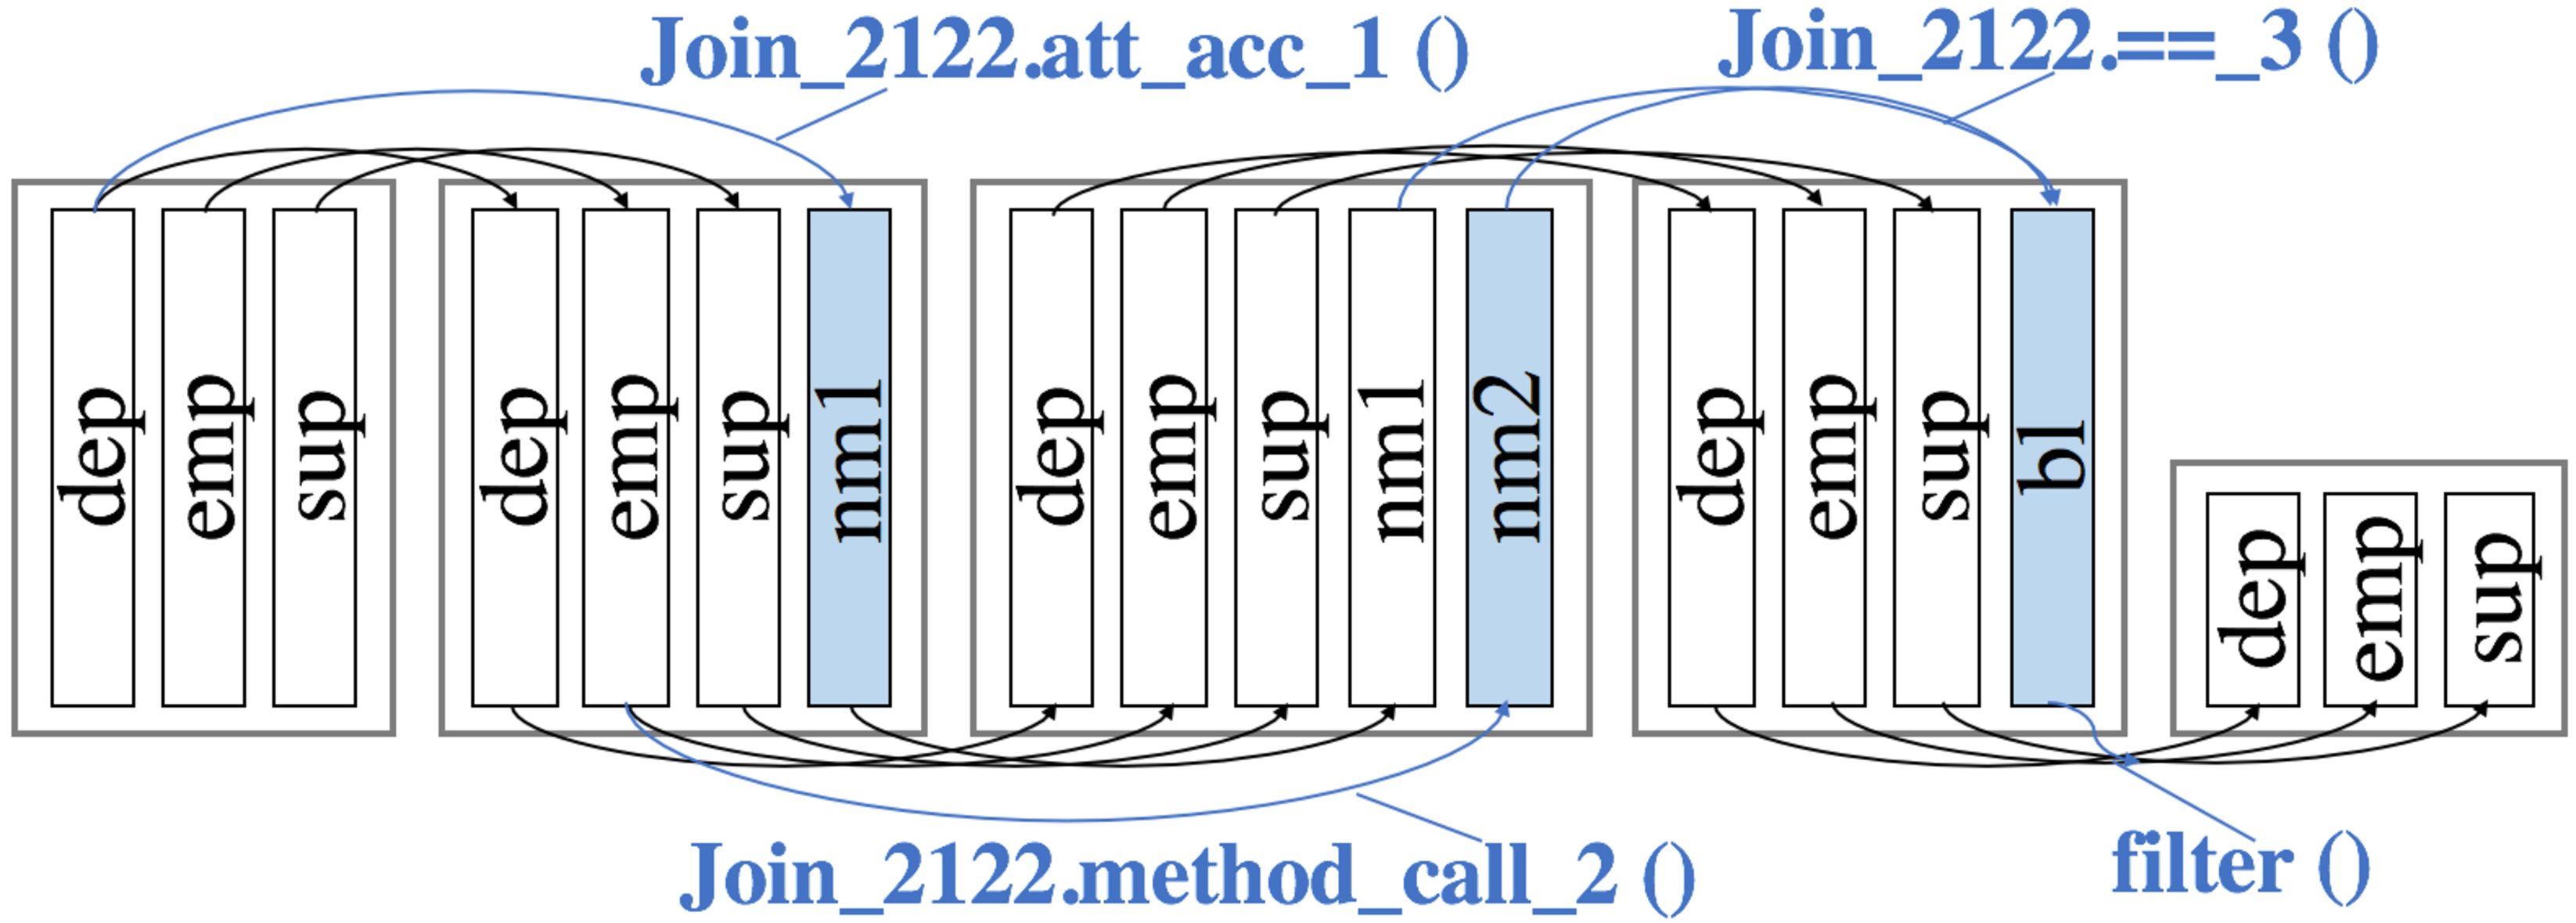
\includegraphics[width=6in]{TCAP}
  \end{center}
\vspace{-10 pt}
  \caption{Execution of the first four stages of a pipeline constructed from the example TCAP program.  The first two stages extract new vectors from 
existing vectors of PC \texttt{Object}s, first via a call to \texttt{Join\_2122.att\_acc\_1 ()}, which extracts \texttt{Dep.deptName} from each item in the vector
\texttt{dep} 
of \texttt{Dep} objects, producing a new vector called \texttt{nm1}. Then, second
via a call to \texttt{Join\_2122.method\_call\_2 ()}, which invokes \texttt{Dep :: getDeptName ()} on each of the \texttt{Emp} objects
in the vector \texttt{emp}, producing a new vector called \texttt{nm2}.  A bit vector \texttt{bl} is formed by checking the equality of those two 
vectors via a call to \texttt{Join\_2122.==\_3 ()}, and then all of the vectors are filtered.}
\vspace{-15 pt}
  \label{fig:TCAP}
\end{figure}


\subsection{TCAP and Vectorized Execution} \label{sec:vectorized}


PC calls the various user-supplied lambda term construction functions for each of the \texttt{Computation} objects in an
input graph, and compiles all of those lambda terms into a DAG of pipeline stages.  
This entire computation is represented using a text-based internal representation that we call
\emph{TCAP} (pronounced ``tee-cap'').  A TCAP program is fully optimizable, using many standard techniques from relational query execution, as we
will discuss subsequently.

As mentioned in Section \ref{sec:engine}, PC's vectorized execution engine repeatedly pushes 
so-called \emph{vector lists} through a series of pipeline stages.  A vector list is (not surprisingly) a list of vectors, where each pipeline stage
takes as input a vector list,
and produces a 
new vector list that consists of zero or more vectors from the input vector list, as well as a new vector or vectors, appended at the end of the list.
Pipeline stages are constructed in such a way that there are no virtual function calls on a per-row basis, aside from any virtual function calls that may be
present (explicitly or perhaps implicitly in the form of memory management) in the user's code.
The TCAP language describes both the pipeline stages required to perform a PC computation, as well as the schema for each of the vector lists that
will be produced during the PC computation, and how each of the pipeline stages add or remove vectors from the vector lists that are pushed through
the computation.

To see how this works through an example, consider a variant of the \texttt{getSelection ()}:

\begin{codesmall} 
Lambda <bool> getSelection (Handle <Dep> arg1, Handle <Emp> arg2, Handle <Sup> arg3) {
	return makeLambdaFromMember (arg1, deptName) == 
	       makeLambdaFromMethod (arg2, getDeptName);  }
\end{codesmall}

\noindent PC compiles the lambda term resulting from a call to \texttt{getSelection ()} into the following TCAP code:

\begin{codesmall}
WDNm_1(dep,emp,sup,nm1) <= APPLY(In(dep), In(dep,emp,sup), 'Join_2212', 'att_acc_1', 
  [('type', 'attAccess'), ('attName', 'deptName')]);

WDNm_2(dep,emp,sup,nm1,nm2) <= APPLY(WDNm_1(emp), WDNm_1(dep,emp,sup,nm1), 'Join_2212',
  'method_call_2', [('type', 'methodCall'), ('methodName', 'getDeptName')]);

WBl_1(dep,emp,sup,bl) <= APPLY(WDNm_2(nm1,nm2),WDNm_2(dep,emp,sup), 'Join_2212', '==_3', 
  [('type', 'equalityCheck')]);

Flt_1(dep,emp,sup) <= FILTER(WBl_1(bl), WBl_1(dep,emp,sup), 'Join_2212', []);
\end{codesmall}

\noindent
These four TCAP statements correspond to a pipeline of four stages,
as shown above in Figure \ref{fig:TCAP}.

This particular TCAP code begins with an \texttt{APPLY} operation, which is a five-tuple, consisting of: (1) the vector list and constituent
vector(s) for the \texttt{APPLY} to operate on, (2) the vector(s) from that vector list to copy
from the input to the output, (3) the name of the computation that the operation was compiled from, (4) the name of the compiled code (pipeline stage)
that the operation is to execute, plus (5) a key-value map that stores specific information about the operation that may be used 
later during optimization.

Specifically, in this case, the first \texttt{APPLY} in the TCAP computation describes the following.  It describes a pipeline stage that
takes as input 
a vector list called \texttt{Input}, which is made of the constituent vectors, referred to using 
the names \texttt{dep}, \texttt{emp}, and \texttt{sup}.
To produce the output vector list (called \texttt{WDNm\_1}), the vectors
\texttt{dep}, \texttt{emp}, and \texttt{sup} should be simply copied (via a shallow copy) from \texttt{In}.
In addition, the compiled code referred to by \texttt{Join\_2212.member\_1} will be executed via a vectorized application to the input
vector \texttt{dep}.  The result will then be put into a new vector called 
\texttt{WDNm\_1.name1}.
The resulting vector list (consisting of the vectors shallow copied from the input as well as the new vector \texttt{WDNm\_1.name1})
will be called \texttt{WDNm\_1}.  

Next, this TCAP program
specifies that \texttt{WDNm\_1} is processed by \texttt{APPLY}ing the
method call \texttt{getDept Name()} on the attribute \texttt{emp}; this is 
done via application of the compiled code referred to by \texttt{Join
  \_2212.method\_call\_1}.  
The vectors \texttt{dep}, \texttt{emp}, \texttt{sup}
and \texttt{nm1} are simply shallow-copied to the output vector set.

After this an equality check is performed to create \texttt{WBl\_1.bl}
(a vector of booleans) and then the result is filtered based upon this
column.


Note that in each TCAP operation, the key-value map is only informational and does not affect the execution of the TCAP.  However, this
information can be vital during optimization.  As we will discuss subsequently, 
multiple calls to the same method can be detected using information stored in TCAP key-value maps, and the redundant calls eliminated.

\subsection{Template Metaprogramming}

In PC,
each vectorized pipeline stage (such as \texttt{Join\_2212.member\_1}) is executed as fully-compiled native code, with no virtual function
calls.
In PC's C++ binding, this is accomplished by using the C++ language's extensive \emph{template metaprogramming} 
capabilities \cite{josuttis2012c++}.  Templates are the C++ language's way of providing generic functionality.
When a C++ template class or
function is instantiated with a type, %the instantiated template 
the C++ compiler actually generates optimized native code for that specific new type, at compile time.  
This is quite different from languages
such as Java, that must typically rely on slow virtual
function calls in order to implement generics.

To see how template metaprogramming is used by PC, consider
the TCAP operation from our example:

\begin{codesmall}
WBl_1(dep,emp,sup,bl) <= 
   APPLY(WDNm_2(nm1,nm2),WDNm_2(dep,emp,sup), 'Join_2212', '==_3', '');
\end{codesmall}

\noindent
Here, the pipeline stage \texttt{Join\_2212.==\_3} that is specified by the \texttt{APPLY} operation
actually refers to a function generated as a by-product of the
programmer using PC's \texttt{==} operation
in the line of code

\begin{codesmall} 
	return makeLambdaFromMember (arg1, deptName) == 
	       makeLambdaFromMethod (arg2, getDeptName); 
\end{codesmall}

\noindent The \texttt{==} 
operation (corresponding to a higher-order function that
constructs a lambda term checking for equality in the output of two input lambda terms) is actually implemented as C++ template
whose two type parameters \texttt{LHSType} and \texttt{RHSType} are inferred from
the output types of the two input lambda terms. 
The \texttt{==} template returns an object of type \texttt{EqualsLambda} \texttt{<LHSType,} \texttt{RHSType>}, which
itself has an operation returning a pointer to the pipeline stage \texttt{Join\_2212.==\_3} referred to in the TCAP.
As expected, this stage processes in an input vector list,
creating a new vector of booleans, containing the truth values of the equality check of each \texttt{LHSType} from the left
input vector and each \texttt{RHSType} from the right input vector.
Using C++'s template metaprogramming facilities, this 
pipeline stage is generated specifically for \texttt{LHSType} and \texttt{RHSType} and optimized by the compiler for use with those
two types.  
As the \texttt{Join\_2212.==\_3} pipeline stage loops over the objects in the input vectors, 
there are no function calls that cannot themselves be inlined by the compiler
and optimized---unless, of course, the (potentially) user-defined equality operation over \texttt{LHSType} and \texttt{RHSType}
objects itself contains a virtual function call.

In this way, each pipeline stage in the graph described by a TCAP program is generated using template metaprogramming.
Actually pushing a vector list through a stage requires no per-data-object virtual function calls, and the pipeline stages
are generated specifically for the types pushed through the pipeline.

\subsection{$k$-Means Example}

Now that we have described PlinyCompute at a high level, we turn to an example of what PlinyCompute looks like to a programmer.

Imagine that a user wished to use PC to build a high-performance library implementation of a $k$-means algorithm.
Once the programmer had defined the basic type over which the clustering is to be performed (such as the
\texttt{DataPoint} class), 
a programmer would likely next define a simple class that allows the averaging of vectors:

\begin{code}
class Avg : public Object {
	long cnt = 1;
	Handle <Vector <double>> data = nullptr;
	Avg &operator + (Avg &addMe) {/* add addMe into this */}
};
\end{code}

\noindent
The programmer might next add a method to the \texttt{DataPoint} class that converts the \texttt{DataPoint} object to an \texttt{Avg} object:

\begin{code}
Avg DataPoint :: fromMe () {
	Avg returnVal;
	returnVal.data = data;
	return returnVal;
}
\end{code}

\noindent
And also add a method to the \texttt{DataPoint} class that accepts a set of centroids, computes the Euclidean distance to
each, and returns the closest:

\begin{code}
long DataPoint :: getClose (Vector <Vector <double>> &centroids) {...}
\end{code}

\noindent
Next, a programmer using PC would define an \texttt{AggregateComp} class using PC's lambda calculus, since, after all, the $k$-means algorithm is essentially 
an aggregation:

\begin{code}
class GetNewCentroids : public AggregateComp <Centroid, long, Avg, DataPoint> {

public:
   Vector <Vector <double>> centroids;

   Lambda <long> getKeyProjection (Handle <DataPoint> aggMe) override {
      return makeLambda (aggMe, [&] (Handle <DataPoint> &aggMe) 
         {return aggMe->getClose (centroids);});
   }
   Lambda <Avg> getValueProjection (Handle <DataPoint> aggMe) override {
      return makeLambdaFromMethod (aggMe, fromMe);
   }
}
\end{code}

\noindent 
The declaration \texttt{AggregateComp <Centroid, long, Avg, DataPoint>} means that this computation aggregates
\texttt{DataPoint} objects.  For each data point, it will extract a key of type \texttt{long}, a value of type \texttt{Avg}, which will be
aggregated into objects of type \texttt{Centroid}.  To process each data point, the aggregation will use the lambdas constructed by
\texttt{getKeyProjection} and \texttt{getValueProjection}.  
In this case, for example,
\texttt{getKeyProjection} builds a lambda which simply invokes the native C++ lambda given in the code---this
native C++ lambda returns the identity of the centroid closest to the data point.

To build a computation using this aggregation class, a programmer would need to specify the \texttt{Centroid} class (the result of this aggregation):

\begin{code}
class Centroid : public Object {
	long centroidId; 
	Avg data;
public:
	long &getKey () {return centroidId;}
	Avg &getVal () {return data;}
};
\end{code}

\noindent
And then build up a computation using these pieces:

\begin{code}
Handle <Computation> myReader = 
    makeObject <ObjectReader <DataPoint>> ("myDB", "mySet");
Handle <Computation> myAgg = makeObject <GetNewCentroids> ();
myAgg->centroids = ... // initialize the model
myAgg->setInput (myReader);
Handle <Computation> myWriter =  makeObject <Writer <Centroid>> ("myDB", "myOutSet");
    myWriter->setInput (myAgg);
pcContext.executeComputations (myWriter);
\end{code}

\noindent After execution, the set of updated centroids would be stored in \texttt{myDB.mySet}.
Performing this computation in a loop, where the centroids are repeatedly updated until convergence, completes the implementation.

In our experience, for many applications such as Linear Algebra
Library, TPCH queries, or KMeans, PC codes require similar work in
terms of lines of source code to develop compared with equivalent codes using Spark's Scala binding, for
example, but require much lower effort to develop than using
object-oriented, C++ code without a declarative interface.

